\chapter{Задача составления рекомендаций}

\section{Входные и выходные данные}

Пусть задано множество пользователей \( U = \{u_1, u_2, \dots, u_m\} \),
множество объектов (предметов) \( I = \{i_1, i_2, \dots, i_n\} \).

Каждый пользователь $u \in U$ может взаимодействовать с некоторыми объектами из $I$.
Взаимодействия могут быть представлены либо явными рейтингами, либо неявными сигналами и могут быть определены
матрицей $R = (R_{u,i})$ размера \( n \times m \), где
\( i \in \{1, \ldots, n\} \) и \( u \in \{1, \ldots, m\} \)~\cite{kut_rec}.


\subsection*{Явная обратная связь}
Предположим, что для некоторой части пар $(u, i) \in U \times I$ известен рейтинг \( R: U \times I \to \mathbb{R} \cup \{0\} \),
где $R \subseteq \mathbb{R}$ -- множество возможных оценок (например, целые числа от 1 до 5), а $\emptyset$ означает отсутствие оценки.

\subsection*{Неявная обратная связь}
Если обратная связь неявная (например, клики, просмотры, покупки), можно также ввести функцию \( R_{u,i} \in \{0, 1\} \),
которая указывает на факт взаимодействия пользователя $u$ с объектом $i$.

\subsection*{Матрица рейтингов}
Пример матрицы рейтингов для явной обратной связи представлен на рисунке~\ref{img:mat}.

\begin{figure}[h]
	\centering
	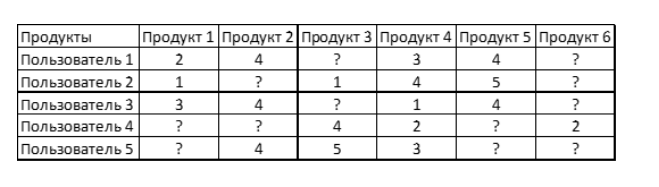
\includegraphics[width=0.8\textwidth]{images/matrix}
	\caption{Матрица рейтингов~\cite{kut_rec}}
	\label{img:mat}
\end{figure}


\subsection*{Выходные данные}
Обозначим через $\hat{R}_{u,i}$ наш прогноз относительно
того, какую оценку пользователь u поставит продукту i. Наша задача
наилучшим образом предсказать, какие оценки $R_{u,i}$ должны стоять на
месте пропусков в матрице рейтингов, то есть рассчитать $\hat{R}_{u,i}$~\cite{kut_rec}.

Затем для каждого пользователя $u$ на основе спрогнозированных оценок $\hat{R}_{u,i}$, нам
нужно сформировать список из $N$ продуктов, которые наиболее точно
удовлетворяют предпочтениям пользователя и не были им
оценены. Список этих $N$ продуктов обозначим через $N$-мерный вектор
\( V = (i_{1}, i_{2}, \ldots, i_{N})\)~\cite{kut_rec}.

\section{Постановка задачи}

Задача рекомендательной системы — максимизировать полезность для пользователей, предсказывая релевантные объекты~\cite{rek_intro}.,
То есть для данного пользователя $u_{i}$ найти \(N\)-мерный вектор \( V = (i_{i_1}, i_{i_2}, \ldots, i_{i_N})\),
где продукты \(i_{i_k}, k \in \{1, \ldots, N\}\) ещё не оценены этим пользователем.
Эту задачу можно представить формулой~\ref{eq:task}, где:
\begin{itemize}
    \item $Range$ — функция ранжирования;
    \item $Relevance$ — функция, измеряющая, насколько хорошо предсказанная оценка $\hat{R}_{u,i}$ соответствует фактическому взаимодействию \( R_{u,i} \).
\end{itemize}

\begin{equation}
    \label{eq:task}
    V = \text{$Range$}(\text{$Relevance$}(\hat{R}_{u,i}, R_{u,i})),
\end{equation}